%
%%%%%%%%%%%%%%%%%%%%%%%%%%%%%%%%%%%%%%%%%%%%%%%%%%%%%%%%%%%%%%%%%%%%%%%%%%%%%%%
% Object reconstruction and event selection
%%%%%%%%%%%%%%%%%%%%%%%%%%%%%%%%%%%%%%%%%%%%%%%%%%%%%%%%%%%%%%%%%%%%%%%%%%%%%%%
%

\chapter{Event reconstruction and \emph{\textbf{b}}-Tagging }\label{ch:reco}


The event reconstruction packages, which in ATLAS are implemented in the software framework {\sc athena}~\cite{Calafiura2005zz}, process the events, starting from the raw data obtained from the various sub-detectors (energy deposits and hits),  %processing them in many 
through different stages to finally interpreting them as a set of charged tracks, electrons, photons, jets, muons and, in general, of possible kinds of final state objects with related four momenta.  
In this chapter the reconstruction of these objects is briefly described together with the algorithms for the identification of $b$-quark jets.  These algorithms are mainly based on the reconstruction of the primary interaction vertex, on the reconstruction of charged particles in the Inner Detector and on the reconstruction of jets in the calorimeter.   

%------------------------------------------------------------------------
\section{Jet reconstruction and calibration}\label{sec:jetcalib}
%------------------------------------------------------------------------

Hadronic jets used for ATLAS analyses are reconstructed by a jet algorithm, starting from the energy depositions of electromagnetic and hadronic showers in the calorimeters. 
%The default jet algorithm is the anti-$k_t$ algorithm, described in Chapter~\ref{ch:theory}. 
The ATLAS performance group, addressing the calibration of jets and the missing transverse energy (Jet/Etmiss), has made the decision to adopt the anti-$k_t$ algorithm (Chapter~\ref{ch:theory}) as its default jet algorithm. This choice was driven by multiple requirements ranging from physics performance to those intimately involved with the computing, trigger and detector: the anti-$k_t$ algorithm is fast and its memory consumption is low, it is well adapted to algorithms used in the trigger, and it has the best jet reconstruction efficiency at low $\pt$. Moreover, this algorithm exhibits the smallest fluctuations of the jet area showing good stability under pile-up~\cite{Asquith:1311867}.
%Due to the expected level of pile-up in the LHC, the primary factor that influenced the selection of this algorithm was the effect of multiple simultaneous interactions on the reconstruction of jets. The original ATLAS cone algorithm, known to contain infrared and collinear sensitivity, is highly susceptible to this effect. On the contrary, the anti-$k_t$ algorithm is the most stable after the introduction of pile-up~\cite{Asquith:1311867}.  

 Two different size parameters are used: $R = 0.4$, for narrow jets, more adecuate to describe the event substructure and associate matrix element partons to jets in multiparton final states; %($t\bar{t}, susy, $W$+jets, etc.)$
and $R = 0.6$, for wider jets, with very little out of cone radiation, more suitable for QCD studies.

The input to calorimeter jet reconstruction can be calorimeter towers or topological cell clusters. Charged particle tracks reconstructed in the Inner Detectors are also used to define jets. The latter have the further advantage of being insensitive to pile-up and they provide a stable reference for systematic studies.
% The jet inputs are combined as massless four-momentum objects in order to form the final four-momentum of the jet, which allows for a well-defined jet mass~\cite{Busato:1271710}. 
Both towers and topological clusters are combined as massless four-momentum objects. In the case of track-jets, the track four-momentum is constructed assuming the $\pi$ meson mass for each track.  The final four-momentum of the jet is obtained from summing the four-momenta of its constituents in the so called ``four-vector recombination scheme''. This scheme conserves energy and momentum and allows a meaningful definition for the jet mass.
In Monte Carlo simulation, reference jets (``truth jets'') are formed from simulated stable particles using the same jet algorithm as for the calorimeter jets. 


Calorimeter towers are static, $\Delta \eta \times \Delta \phi = 0.1 \times 0.1$, grid elements built directly from calorimeter cells. There are two types of calorimeter towers: with or without noise supression. The latter are called ``noise-suppressed'', %towers 
and use only the cells with energies above a certain noise threshold.  The noise of a calorimeter cell is measured by recording calorimeter signals in periods where no beam is present in the acelerator.  The standard deviation $\sigma$ around the mean %measured 
no-beam energy is interpreted as the noise of the cell, and it depends on the sampling layer in which the cell resides and the position in $\eta$.

The results presented in this thesis use jets built from noise-suppressed topological clusters,  %of energy in the calorimeter, 
also known as ``topo-clusters''~\cite{topoClusters}. Topological clusters are groups of calorimeter cells that are designed to follow the shower development taking advantage of the fine segmentation of the ATLAS calorimeters. The topological cluster formation starts from a seed cell with $|E_{cell}| > 4 \sigma$ above the noise. In a second step, neighbor cells that have an energy at least 2$\sigma$ above their mean noise are added to the cluster. Finally, all nearest-neighbor cells surrounding the clustered cells are added to the cluster, regardless of the signal-to-noise ratio\footnote{Noise-supressed towers also make use of the topological clusters algorithm~\cite{topoClusters} to select cells, i.e. only calorimeter cells that are included in topo-clusters are used.}. The position of the cluster is assigned as the energy-weighted centroid of all constituent cells (the weight used is the absolute cell energy).


\subsubsection{Jet calibration}\label{sec:calib}

The baseline EM energy scale of the calorimeters is the result of the calibration of the electronics signal to the energy deposited in the calorimeter by electromagnetic showers (see Chapter~\ref{ch:lhc_atlas}).
The purpose of the jet energy calibration, or jet energy scale (JES), is to correct the measured EM scale energy to the energy of the stable particles within a jet.  The jet energy calibration must account then for the calorimeter non-compensation; the energy lost in inactive regions of the detector, such as the cryostat walls or cabling; energy that escapes the calorimeters, such as that of highly-energetic particles that ``punch-through'' to the muon system; energy of cells that are not included in clusters, due to inefficiencies in the noise-suppression scheme; and energy of clusters not included in the final reconstructed jet, due to inefficiencies in the jet reconstruction algorithm. The muons and neutrinos that may be present within the jet are not expected to interact within the calorimeters, and are not included in this energy calibration.
Due to the varying calorimeter coverage, detector technology, and amount of upstream inactive material, the calibration that must be applied to each jet to bring it to the hadronic scale varies with its $\eta$ position within the detector. 
%The jet energy is first reconstructed from the constituent cell energies at EM scale. These cells have been calibrated to return the energy corresponding to electromagnetic showers in the calorimeter, based on test-beam injection of electrons and pions~\cite{Aharrouche2006601},  measurements of cosmic muons~\cite{Cooke:1071187} and the reconstruction of the $Z$ mass peak in $Z \rightarrow ee$ decays~\cite{Aad:2011mk}. The correction for the lower response to hadrons is based on the topology of the energy depositions observed in the calorimeter. 

A number of complex calibration schemes, taking into account these effects, have been developed in ATLAS. The simplest procedure used for 2011 data, referred to as ``EM+JES'' calibration, utilizes an energy and $\eta$-dependent calibration scheme that is primarily based on Monte Carlo simulation with some direct in-situ measurements. This is the calibration used in this thesis. It consists of three subsequent steps:

%In the simplest case the measured jet energy is corrected, on average, using Monte Carlo simulations, as follows:
%
%\begin{equation}
%E^{jet}_{calib} = E^{jet}_{meas} /\mathcal{F}_{calib}(E^{jet}_{meas}),\; \; \mbox{with} \;  E^{jet}_{meas} = E^{jet}_{EM} - \mathcal{O}(\mbox{NPV}),
%\end{equation}
%
%where $E^{jet}_{EM}$ is the calorimeter energy measured at the electromagnetic scale, $E^{jet}_{calib}$ is the calibrated energy and $\mathcal{F}_{calib}$ is the calibration function that depends on the measured jet energy and is evaluated in small jet $\eta$ regions. The variable $ \mathcal{O}(\mbox{NPV})$ denotes the correction for additional energy from multiple proton-proton interactions depending on the number of primary vertices (NPV).

 

\begin{itemize}
\item
Pile-up correction: An offset correction is applied in order to substract the additional average energy measured in the calorimeter due to multiple proton-proton interactions. This correction is derived from minimum bias data %using events from a trigger stream containing triggers for all calorimeter objects
 as a function of NPV, the jet pseudorapidity and the bunch spacing. This additional energy is substracted before the hadronic energy scale is restored such that the derivation of the jet energy scale calibration is factorized and does not depend on the number of interactions in the event.
\item
Vertex correction: The jet four momentum is corrected such that the jet originates from the primary vertex of the interaction instead of the geometrical centre of the detector. 
\item
Jet energy and direction correction: The jet energy and direction are corrected using constants derived from the comparison of the kinematic observables of reconstructed jets and those from truth jets in the simulation.
\end{itemize}

In the final step the calibration is derived in terms of the energy response of the jet, or the ratio of the reconstructed jet energy to that of a ``truth'' jet built of all truth stable interacting particles in the Monte Carlo. This response, written as
%
\begin{equation}
\mathcal{R} = E_{reco} / E_{truth}
 \label{eqn:response}
\end{equation}
%
may be defined at any energy scale. In Equation~\ref{eqn:response}, $E_{truth}$ is the energy of the closest isolated truth jet, within $\Delta R < 0.3$\footnote{This value was chosen because it results in a reconstructed-to-truth jet match more than 99\% of the times.}.
The isolation requirement is applied in order to factorize the effects due to close-by jets from those due to purely detector effects such as dead material and non-compensation. The isolation criterion requires that no other jet with a $\pt > 7$~GeV be within $\Delta R < 2.5R$, where $R$ is the distance parameter of the jet algorithm.

 The jet energy response is binned in truth jet energy and the calorimeter jet $\eta$.  For each $(E_{truth}, \eta)$-bin, the averaged jet energy response is defined as the peak position of a Gaussian fit to the $E_{reco} / E_{truth}$ distribution. The jet $\pt$ response, which will be used later, uses the $\pt^{reco} / \pt^{truth}$ distribution.


The EM+JES calibration constants consist in the inverse of the response: $\mathcal{C}(\pt^{EM})=\mathcal{R}^{-1}_{reco}(\pt^{EM})$, where $\mathcal{C}$ is the calibration constant and $\mathcal{R}_{reco}$ is the response calculated as a function of reconstructed jet $\pt$. They are derived as a function of $\pt^{truth}$, to remove the impact of the underlying $\pt$ spectrum on the response.  The jet response determined as a function of $\pt^{truth}$, $\mathcal{R}_{truth}$, is used to apply the constants as a function of $\pt^{EM}$, that is $\mathcal{R}_{reco}(\pt^{EM})=\mathcal{R}_{truth}(\mathcal{R}_{truth}\cdot \pt^{truth})$. This relationship is valid in ATLAS due to the linearity of the jet response as a function of $\pt$.
The correct energy scale is obtained by multiplying the EM scale energy of a jet by  the calibration constant 
%
\begin{equation}
%E^{jet}_{EM+JES} = \frac{E^{jet}_{EM}}{\mathcal{F}_{calib}(E^{jet}_{EM})|_{\eta}},
E^{EM+JES} = \mathcal{C} \cdot E^{EM}.
\end{equation}
%

%A function $\mathcal{F}_{calib,k}(E^{jet}_{EM})$ is then defined for each $\eta$-bin $k$ that describes the response as a function of the uncalibrated jet energy. $\mathcal{F}_{calib,k}(E^{jet}_{EM})$ is parameterised as:
%%
%\begin{equation}
%\mathcal{F}_{calib,k}(E^{jet}_{EM}) = \sum_{i=0}^{N_{max}} a_{i,k} (\ln E^{jet}_{EM})^i,
%\end{equation}
%%
%where $a_i$ are free parameters, and $N_{max}$ is chosen between 1 and 6 depending on the goodness of the fit. 
%The final jet energy scale correction that relates the jet energy measured at EM scale to the hadronic scale is then  % defined as $1/\mathcal{F}_{calib,k}(E^{jet}_{EM})$ in the following:
%
%\begin{equation}
%E^{jet}_{EM+JES} = \frac{E^{jet}_{EM}}{\mathcal{F}_{calib}(E^{jet}_{EM})|_{\eta}},
%E^{EM+JES} = \mathcal{C}E^{EM}.
%\end{equation}
%
%where $\mathcal{F}_{calib}(E^{jet}_{EM})|_{\eta}$  is $\mathcal{F}_{calib,k}(E^{jet}_{EM})$ for the relevant $\eta$-bin $k$.


Other calibrations schemes are the global calorimeter cell weighting (GCW) calibration and the local cluster weighting (LCW) calibration.  The GCW scheme exploits the observation that electromagnetic showers in the calorimeter leave more compact energy depositions than hadronic showers with the same energy.  Energy corrections are derived for each cell within a jet.  The cell corrections account for all energy losses of a jet in the detector. Since these corrections are only applicable to jets and not to energy depositions, they are called ``global'' corrections.

The LCW calibration method first classifies topo-clusters as either electromagnetic of hadronic, based on the measured energy density. Energy corrections are derived according to this classification from single charged and neutral pion Monte Carlo simulations. Dedicated corrections are derived for the effects of non-compensation, signal losses due to noise threshold effects, and energy lost in non-instrumented regions. Since the energy corrections are applied without reference to a jet definition they are called ``local'' corrections. Jets are then built from these calibrated clusters using a jet algorithm.  

%The final jet energy calibration can be applied to EM scale jets, with the resulting calibrated jets referred to as EM+JES, or to LCW (GCW) calibrated jets, with the resulting jets referred to as LCW+JES (GCW+JES) jets.

A further jet calibration scheme called global sequential (GS) calibration, starts from jets calibrated with the EM+JES calibration and corrects the energy jet-by-jet, without changing the average response. This scheme exploits the topology of the energy deposits in the calorimeter to characterize fluctuations in the jet particle content of the hadronic shower development.  Correcting for such fluctuations can improve the jet energy resolution. The correction uses several jet properties, and each correction is applied sequentially.


For the 2011 data the recomended calibration schemes were the EM+JES and the LCW calibrations. The simple EM+JES calibration does not provide the best resolution performance, but allows in the central detector region the most direct evaluation of the systematic uncertainties from the calorimeter response to single isolated hadrons measured \emph{in situ}  and in test-beams and from systematic variations in the Monte Carlo simulation.  For the LCW calibration scheme the JES uncertainty is determined from \emph{in situ}  techniques. For all calibration schemes, the JES uncertainty in the forward regions is derived from the uncertainty in the central region using the transverse momentum balance in events where only two jets are produced. 



\subsubsection{Jet energy scale uncertainties for the EM+JES scheme}

For many physics analyses, the uncertainty on the JES constitutes the dominant systematic uncertainty because of its tendency to shift jets in and out of analysis selections due to the steeply falling jet $\pt$ spectrum. The uncertainty on the EM+JES scale  is determined primarily by six factors:  varying the physics models for hadronization and parameters of the Monte Carlo generators, evaluating the baseline calorimeter response to single particles, comparing multiple models for the detector simulation of hadronic showers, assesing the calibration scales as a function of pseudorapidity, and by adjusting the JES calibration methods itself.  The final JES uncertainty in the central region, $|\eta| < 0.8$, is determined from the maximum deviation in response observed with respect to the response in the nominal sample.  For the more forward region, the so called ``$\eta$-intercalibration'' contribution is estimated. This is a procedure that uses direct di-jet balance measurements in two-jet events to measure the relative energy scale of jets in the more forward regions compared to jets in a reference region. The technique exploits the fact that these jets are expected to have equal $\pt$ due to transverse momentum conservation. Figure~\ref{fig:JESuncertainty}  shows the final fractional jet energy scale uncertainty and its individual contributions as a function of $\pt$ for a central $\eta$ region. The JES uncertainty for anti-$k_t$ jets with $R = 0.4$ is between $\approx$4\% (8\%, 14\%) at low jet $\pt$ and $\approx$2.5\%-3\% (2.5\%-3.5\%, 5\%) for jets with $\pt > 60$~GeV in the central (endcap, forward) region.

\begin{figure}[htbp]
  \begin{center}
   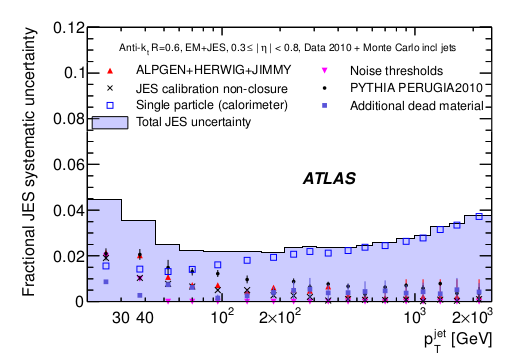
\includegraphics[width=0.9\textwidth]{JESUncertainty.png}
    \caption{Fractional jet energy scale uncertainty as a function of jet $\pt$ for jets in the pseudorapidity region 0.3$ < |\eta| < $0.8 in the calorimeter barrel. The total uncertainty is shown as the solid tight blue area. The individual sources are also shown.}
    \label{fig:JESuncertainty}
  \end{center}
\end{figure}

In addition to the tests above, \emph{in situ} tests of the JES using direct $\gamma$-jet balance, multi-jet balance, and track-jets indicate that the uncertainties in Fig.~\ref{fig:JESuncertainty} reflect accurately the true uncertainties in the JES.  

In the case of jets induced by bottom quarks ($b$-jets), the calorimeter response uncertainties are also evaluated using single hadron response measurements \emph{in situ}  and in test beams~\cite{ATLAS-CONF-2011-028}. For jets within $|\eta|<0.8$ and $20 \leq \pt < 250$~GeV the expected difference in the calorimeter response uncertainty of identified $b$-jets with respect to the one of inclusive jets is less than 0.5\%. It is assumed that this uncertainty extends up to $|\eta| < 2.5$.
% Single hadrons with momenta up to 20GeV are selected in minimum bias sample produced in pp collisions at 7TeV taken in 2011 and the calorimeter energy (E) in a narrow cone around an isolated track is compared to the track momentum (p). In this method, jets are treated as a superposition of energy deposits of single particles. For each calorimeter deposition within the jet cone, the type of the particle inside the jet is determined and the expected mean shift and the systematic uncertainty of the calorimeter response between data and monte carlo simulation is evaluated.

The JES uncertainty arising from the modelling of the $b$-quark fragmentation can be determined from systematics variations of the Monte Carlo simulation. The fragmentation function is used to estimate the momentum carried by the $b$-hadron with respect to that of the $b$-quark after quark fragmentation.   The fragmentation function included in {\sc pythia} originates from a detailed study of the $b$-quark fragmentation function in comparison with OPAL~\cite{Abbiendi:2002vt} and SLD~\cite{Abe:2002iq} data. To assess the impact of the $b$-fragmentation, the nominal parameters of the {\sc pythia} fragmentation function are replaced by the values from a tune using the Professor framework~\cite{Professor}. In addition, the nominal fragmentation function is replaced by the modified Bowler-Lund fragmentation function~\cite{BowlerLund}. The $b$-jet response uncertainty is evaluated from the ratio between the response of $b$-jets in the varied Monte Carlo samples to the nominal {\sc pythia}. The response variations are well within 2\%.

The $b$-jet JES uncertainty is obtained adding the calorimeter response uncertainty and the uncertainties from the systematic Monte Carlo variations in quadrature. The resulting additional JES uncertainty for $b$-jets is shown in Fig.~\ref{fig:bjetJESuncertainty}. It is about 2\% up to $\pt \approx 100$~GeV and below 1\% for higher $\pt$. To obtain the overall $b$-jet uncertainty this uncertainty is added in quadrature to the JES uncertainty for inclusive jets.

\begin{figure}[htbp]
  \begin{center}
      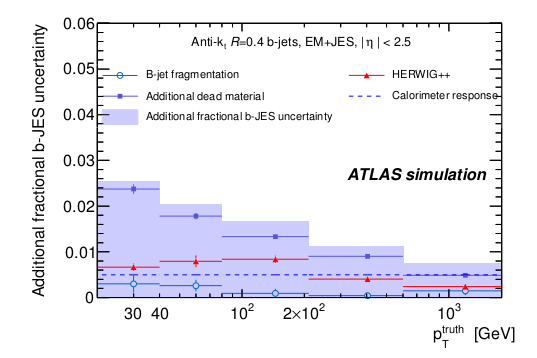
\includegraphics[width=0.9\textwidth]{bjetsJESUncertainty.png}
    \caption{Additional fractional $b$-jet JES uncertainty as a function of the truth jet transverse momentum for anti-$k_t$ jets with $R=0.4$ calibrated with the EM+JES scheme for $|\eta| < 2.5$. Shown are systematic Monte Carlo variations using different modelling of the $b$-quark fragmentation and physics effects as well as variations in the detector geometry and the uncertainty in the calorimeter response to $b$-jets as evaluated from single hadron response measurements.  Uncertainties in the individual points are statistical only. }
    \label{fig:bjetJESuncertainty}
  \end{center}
\end{figure}


%-------------------------------------------------------------------
\section{Reconstruction of charged particle tracks}\label{sec:trackreco}
%------------------------------------------------------------------------

The Inner Detector layout and the characteristics of its main sub-detectors were presented in Section~\ref{atlasID} of Chapter~\ref{ch:lhc_atlas}. The algorithm used for track reconstruction is based on a modular software framework, which is described in more detail in Ref.~\cite{Cornelissen:1020106}. The main steps are the following:

\begin{itemize}
\item
Firstly, the raw data from the pixel and SCT detectors are converted into clusters, while the TRT raw timing information is turned into calibrated drift circles. The SCT clusters need to be further transformed into space-points, by combining the clusters information from opposite sides of the SCT module (stereo strip layers).
\item
In a second stage, the track-finding is performed, in which the pattern recognition and a global $\chi^2$ minimization procedure is implemented as a default.
\end{itemize}

In the track-finding stage, track seeds are found in the first three pixel layers and in the first SCT layer. These are extended throughout the SCT to form track candidates and a first track fit is performed. Afterwards, ambiguities in the track candidates found in the silicon detectors are resolved, and tracks are extended into the TRT (which covers up to $|\eta|<2.$, while Pixel and SCT cover up to 2.5). The final track candidate is refitted with the full information from the three tracking subdetectors. The baseline algorithm is designed for the efficient reconstruction of primary charged particles. Primary particles are defined as particles with a meanlife of greater than $3 \times 10^{-11}$~s directly produced in a proton-proton interaction, or from the subsequent decays or interactions of particles with lifetime shorter than $3 \times 10^{-11}$~s. The tracks reconstructed in this stage are required to have $\pt> 400$~MeV.

In a complementary stage, a track search starts from segments reconstructed in the TRT and extends them inwards by adding silicon hits, which is referred to as ``back-tracking''. This recovers tracks for which the first hits in the pixel layers are missing, e.g. because they originate from secondaries, which are produced in decays or the interaction of primaries.

The final reconstructed track trajectory is usually specified at its closest point to the interaction region on the transverse plane by its impact parameters in the transverse plane and in the longitudinal direction, respectively called $d_0$ and $z_0$\footnote{Stricktly speaking the impact parameter is $|z_0|sin\theta$, where $\theta$ is the polar angle of the track.}, and by its momentum, typically expressed in azimuthal angle $\phi$, polar angle $\theta$ and inverse momentum $1/p$. 

 The track reconstruction efficiency is defined as the fraction of primary particles with $\pt> 400$~MeV and $|\eta|<2.5$ matched to a reconstructed track. The reconstruction efficiency for primary tracks with transverse momentum above 1~GeV and central $\eta$ is above 80\%, going down to values below 70\% for tracks at the edge of the Inner Detector acceptance~\cite{chargemultiplicity}. %REFERENCIAS?
The dense environment of a jet decreases the track reconstruction efficiency and increases the fake rate. This is caused by the ocurrence of shared hits between different tracks, which makes the pattern recognition and track fitting tasks more difficult.

The relative transverse momentum scale and resolution of tracks is defined as the Gaussian mean and width of
%
\begin{equation}
\pt^{MC} \times (1/\pt^{MC}  - 1/\pt^{reco}) = 1 - \frac{\pt^{MC}}{\pt^{reco}}
\end{equation}
%
where $\pt^{MC}$ ($\pt^{reco}$), refers to the track's transverse momentum given by simulation truth (MC) or by reconstruction (reco). It should be noted that the ($1/\pt$) resolution is used instead of $\sigma(\pt)$ as the Inner Detector measures the sagitta and not directly the transverse momentum\footnote{The relation between sagitta $s$ and transverse momentum ($\pt$) is given by $s \sim  1/\pt$. }.  However, the resolution obtained from the equation above is the relative transverse momentum resolution,  $\sigma(\pt) / \pt$. At low $\pt$ the multiple scattering dominates the resolution, and at high momenta, the resolution is limited by the bending power of the solenoid field and by the instrinsic detector resolution.  For a central track with $\pt=$5~GeV %, which is typical for $b$-tagging, 
the transverse momentum resolution is around 75~MeV and the transverse impact parameter resolution is about 35~$\mu$m.



%-------------------------------------------------------------------
\section{Vertex reconstruction}\label{sec:trackreco}
%------------------------------------------------------------------------

Primary vertices are reconstructed using an iterative vertex finding algorithm~\cite{ATLAS-CONF-2010-069}. In a first step, a dedicated vertex finding algorithm associates tracks to vertex candidates. Vertex seeds are obtained by looking for the global maximum in the distribution of the $z$ coordinates of the tracks. In a second stage, an iterative $\chi^2$ fit is made using the seed and nearby tracks. Each track carries a weight which is a measure of its compatibility with the fitted vertex depending on the $\chi^2$ of the fit. Tracks displaced by more than 7$\sigma$ from the vertex are used to seed a new vertex and the procedure is repeated until no additional verteces can be found.  %During reconstruction vertices are required to contain at least two tracks.
The parameters of the beam spot are used both during the finding to preselect compatible tracks and during the fitting step to constrain the vertex fit.


The knowledge of the position of the primary interaction point (primary vertex) of the proton-proton collision is important for $b$-quark jets identification since it defines the reference point with respect to which impact parameters and vertex displacements are measured.  The typical vertexing resolution in $z$ is $\mathcal{O}$($100 \mu$m).


To ensure a good resolution on the vertex position, the primary vertex
must be reconstructed from at least five tracks. The choice of the primary vertex is less trivial in the presence of minimum-bias events from pile-up:
the primary vertex from a pile-up event may be mistakenly used as the signal vertex, or a fake primary vertex built from tracks from two different vertices may be reconstructed. The current strategy is to choose the primary vertex candidate that maximizes $\sum_{tracks} \pt^2$.

%-------------------------------------------------------------------
\section{ $b$-jet Tagging}\label{sec:btagging}
%------------------------------------------------------------------------

%From Gbb note
%Jets are classified as $b$-quark candidates by the ATLAS MV1 $b$-tagging algorithm, based on a neural network that combines the information from three high-performance taggers: IP3D, SV1 and JetFitter \cite{ATLAS-CONF-2011-102}.  These three tagging algorithms use a likelihood ratio technique in which input variables are compared to smoothed normalized distributions for both the $b$- and background (light- or in some cases $c$-jet) hypotheses, obtained from Monte Carlo simulation.  The IP3D tagger takes advantage of the signed transverse and longitudinal impact parameter significances. The SV1 tagger reconstructs an inclusive vertex formed by the decay products of the $b$-hadron and relies on the invariant mass of all tracks associated to the vertex, the ratio of the sum of the energies of the tracks in the vertex to the sum of the energies of all tracks in the jet and the number of two-track vertices. The JetFitter tagger exploits the topology of the primary, $b$- and $c$-vertices and combines vertex variables with the flight length significance.  The $b$-tagging performance is determined using a simulated $t\bar{t}$ sample and is calibrated using experimental data with jets containing muons and with a sample of $t\bar{t}$ events~\cite{ATLAS-CONF-2011-089}.


The ability to identify jets originating from $bottom$-quarks (denoted as $b$-tagging in the following) is important for the high-$\pt$ physics program of a general-purpose experiment at the LHC such as ATLAS since many interesting physics processes contain $b$-quarks in the final state, while the most abundant backgrounds contain mostly up, down and strange quark or gluon jets or, in a smaller fraction of cases, charm quark jets. The aim of $b$-tagging is therefore to identify the $b$-quark jets with high efficiency, while rejecting most of the background contamination from jets originating from the fragmentation of light ($u$, $d$, and $s$) quarks, gluons and $c$-quarks.

A $b$-quark, once produced, fragments necessarily into a $b$-flavoured hadron, $b$-hadron in the following. In most of the cases ($\approx$87\%), first an excited $b$-hadron is produced, like a $B^{*}$ or a $B^{**}$, which decays inmediately, strongly or electromagnetically, into a ground state $b$-hadron plus one or more further particles; while in the remaining cases, a ground state $b$-hadron is produced directly.  One is only interested in the transition from a $b$-quark into the final state $b$-hadron, since the typical timescale for electromagnetic or strong interactions is so small that the  $B^{*}$, $B^{**}$ decay vertices are not significantly displaced with respect to the primary vertex.   In most of the cases ($\approx$ 91\%) a $b$-meson is produced out of the fragmentation of an original $b$-quark (40\% $B^+$, 40\% $B^0$ and 11\% $B^0_s$). The rest are $b$-baryons.

Due to the $b$-quark fragmentation function being very hard, most of the original $b$-quark energy is transmitted to the final $b$-hadron. This fraction is for example 70\% for $b$-quarks with a momentum of $\approx$45~GeV. This property can be exploited during $b$-tagging, since the fragmentation for light quarks into light hadrons or $c$-quarks into $c$-hadrons is softer.

Any of the finally produced $b$-hadrons decay through weak interactions and therefore have a significant lifetime, which is on average, for all $b$-hadrons considered, $(1.568\pm0.009) \times 10^{-12}$~s.  The effective distance travelled in the detector by the $b$-hadron before decaying depends on the $b$-hadron momentum, which enters the relativistic boost factor $\beta\gamma$. A $b$-quark with momentum of 50~GeV will travel around 3~mm, which is a visible flight length in the detector. Due to the combination of the $b$-hadron lifetime and relatively high mass ($m_B \approx 5.28$~GeV), which results in a non-negligible decay angle of the $b$-hadron decay products %PUEDO EXPLICAR ESTO?
with respect to the $b$-hadron flight direction, the charged particles produced at the decay vertex will be on average significantly displaced with respect to the primary vertex position.

This is the main signature which is exploited by the \emph{lifetime} based $b$-tagging algorithms, which depend either on the presence of significantly displaced tracks, as in impact parameter based $b$-tagging algorithms, or on the explicit reconstruction of the $b$-hadron decay vertex, as in secondary vertex based $b$-tagging algorithms.


$b$-hadrons decay preferably into a $c$-hadron plus additional particles\footnote{Weak decays are governed by the CKM matrix mechanism, and $|V_{cb}|^2 >> |V_{ub}|^2$.}. The lifetime of a $c$-hadron is not much lower than for $b$-hadrons, but in general the momentum of the $c$-hadron will be lower than the original $b$-hadron momentum. However, the $c$-hadron can still travel for a significant path in the detector and form with its decay producs a visible $tertiary$ vertex. 
%MORE ON C-HADRONS HERE OR LATER??
%There are several strategies to deal with tertiary vertices from $c$-hadron decays. In the case of $b$-tagging algorithms based purely on impact parameter information from charged particle tracks, the presence of tracks with a more significant displacement  does not require an explicit strategy: these tracks will in general improve the $b$-tagging performance. In the case of a secondary vertex based $b$-tagging algorithm, the more conventional approach is to tray to find a single inclusive secondary vertex, which will result in a weighted average of the $b$- and one or more $c$-hadron vertex posotions. This approach is reasonable, since in most of the cases either the resolution of the tracks or the decay vertex multiplicities at such vertices do not allow to separate them efficienctly. An alternative approach instead tries to resolve the $b$- and $c$-hadron decay vertices.

Another property which is usually exploited by $b$-tagging is the fraction of $b$- and $c$-hadron decays into leptons: a lepton from the semi-leptonic decay of a $b$-hadron ($b \rightarrow l$) or from the subsequent $c$-hadron decay ($b \rightarrow c \rightarrow l$) is produced in $\approx$21\% of the cases. This is valid both in case the lepton is a an electron or a muon, which brings the overall fraction of $b$-quarks ending up into final state containing  a lepton to $\approx$42\%. Due to the $b$- or $c$-hadron mass, the lepton will be emitted with an average transverse momentum comparable with $m_{b-had}$ or $m_{c-had}$. By identifying either an electron or a muon originating from a jet and by requiring it to have sufficiently high $\pt$ with respect to the jet axis, it is possible to identify $b$-jets.



\subsubsection{Association of tracks to jets}

The $b$-tagging performance relies critically on the accurate reconstruction of the charged tracks in the ATLAS Inner Detector.  The actual tagging is performed on the sub-set of tracks in the event that are associated to jets.  The $b$-tagging algorithm takes as input the three-momenta of the jets, reconstructed by a jet algorithm, and uses the jet direction to associate the charged particles tracks to the jet. Since the 2 Tesla solenoidal magnetic field of the ATLAS Inner Detector bends charged particles in the transverse plane, in particular in the case of low $\pt$ tracks, the tracks are best matched to the jet by using the direction of their momenta at the point of closest approach to the interaction region.  The criterion for associating charged particle tracks to jets is simply:
%
\begin{equation}
\Delta R(jet, track) < \Delta R_{cut}
\end{equation}
%
where usually the value of $\Delta R_{cut} = R$ is used; with $R$, the distance parameter of the jet algorithm used for jet reconstruction.

After the tracks are associated to the jets, they are filtered in order to remove tracks with bad quality or which can easily be erroneously identified as secondary tracks from $b$-decays. These include tracks originating from decays of even longer lived particles, like $K^0_s$ (c$\tau \approx$2.69~cm) and $\Lambda$ baryons (c$\tau \approx$7.89~cm); from electromagnetic interactions in the detector material, like conversions in electron-positron pairs ($\gamma \rightarrow e^+ e^-$); or from hadronic interactions with the detector material, which result in two or more tracks with high impact parameter. 
In order to reject badly reconstructed tracks, quality cuts are applied. Requirements are imposed on the number of silicon hits, the track fit quality,  the track momentum, and the transverse and longitudinal impact parameters. The track selection needs to be particularly tight in the case of the impact parameter based $b$-tagging algorithms, since in that case the explicit presence of a vertex is not required, so that the influence of badly reconstructed tracks or tracks from long lived particles does directly limit the performance. The minimum track $\pt$ required is of 1~GeV in the case of the impact parameter based algorithms and of 400-500~MeV otherwise. The transverse and longitudinal
impact parameters must fulfill  $|d_0|<$1~mm (3.5~mm) and $|z_0| \sin \theta < 1.5$~mm (no cut on $z_0$) in the case of the algorithms relying on the impact parameters of tracks (on the reconstruction of secondary vertices).  The minimum number of precision hits required is typically 7, for both approaches. 





\subsection{$b$-tagging algorithms}

For the 2011 data-taking a set of lifetime taggers were commissioned and calibrated. In this section a brief description of the main features of these algorithms will be given. 

\subsubsection{Impact parameter based $b$-tagging algorithms }

% AQUI PLOTS OF TRACK PROPERTIES IN JETS???????????

The charged particle tracks originating from $b$-hadrons are expected to have significantly higher transverse and longitudinal impact parameters compared to prompt tracks originating directly from fragmentation. If the effect of long lived particles, conversions and hadronic interactions can be reduced, the best discrimination between prompt tracks and displaced tracks from $b$- and $c$-hadron decays can be obtained using the impact parameter significance, both in the transverse and longitudinal plane. With
%
\begin{equation}
    IP_{r\phi} = d_0\;\;  \mbox{and} \;\;  IP_{z} = z_0 \sin \theta,
\end{equation}
%
the transverse and longitudinal impact parameter significances are obtained by dividing $IP_{r\phi}$ and $IP_z$ by their respective errors,
\begin{equation}
    IP_{r\phi}/\sigma(IP_{r\phi})\;\; \mbox{and} \;\;  IP_{z}/\sigma(IP_{z}).
\end{equation}
%

On the basis that the decay point of the $b$-hadron must lie along its flight path, and in order to increase the discriminating power of the impact parameter significance, a lifetime sign is assigned to these variables (replacing the sign of the geometrical definition of the impact parameter). The sign is positive if the track extrapolation crosses the jet direction in front of the primary vertex (i.e. is more compatible with having its origin in a secondary decay vertex in the direction of flight expected for the $b$-hadron) or negative if the track is more likely to intersect the flight axis behind the primary vertex, opposite to the jet direction. Both cases are illustrated in Fig.~\ref{fig:signedIP}. 

\begin{figure}[htbp]
  \begin{center}
      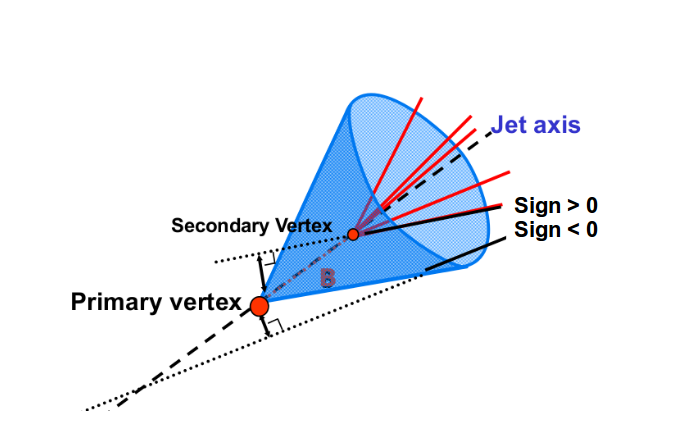
\includegraphics[width=0.7\textwidth]{signedFinal.png}
    \caption{Lifetime sign of tracks. A positive and a negative lifetime signed track is shown.}
    \label{fig:signedIP}
  \end{center}
\end{figure}

%more formal definition of the sign
The lifetime sign can be defined in three-dimensions, acording to the variables $\vec{\pt}_{jet}$, $\vec{\pt}_{trk}$ and $\vec{\Delta r}_{IP} = \vec{r}_{IP} = \vec{r}_{PV}$, the three-dimensional impact parameter of the track with respect to the primary vertex:
%
\begin{equation}
\mbox{sign}_{3D} = \mbox{sign}([\vec{p}_{trk} \times \vec{p}_{jet}]\cdot[\vec{p}_{trk} \times \vec{\Delta r}_{IP} ]).
\end{equation}
%
The computation of the lifetime sign assumes that the jet direction reproduces, up to a good approximation, the $b$-hadron direction. Under this assumption and up to resolution effects both on the jet direction and on the impact parameter and momentum of the track, the lifetime sign of tracks originating from $b$-hadron decays is positive.

The lifetime sign can also be defined on the transverse plane $(x-y)$ or on the longitudinal plane $(r\phi-z)$ by considering respectively the transverse and longitudinal impact parameters (the projections of the three-dimensional impact parameter on the respective planes):
%
\begin{equation}
\mbox{sign}_{r\phi} = \mbox{sign}(\sin(\phi_{jet} - \phi_{trk})\cdot d_{0,trk}); \; \mbox{and} \; \mbox{sign}_{z} = \mbox{sign}((\eta_{jet} - \eta_{trk})\cdot z_{0,trk}).
\end{equation}
%
%PLOTS TO DO
%%%%Extra info
%The definition for sign$_{r\phi}$ compared to sign$_{3D}$ shields to a more positive shifted distribution for tracks from $b$-hadron decays, and thus potentially a better performance. This result is a bit surprising and seems to indicate that, since the lifetime sign is not taking into account the different errors on the longitudinal and transverse impact parameters, the longitudinal component of the lifetime sign is diluting the information from the transverse component.
Distributions of the signed transverse impact parameter and signed transverse impact parameter significance for light, $c$-, and $b$-jets, are shown in Fig.~\ref{fig:IPsignificance} for experimental data and for simulation; the sign %of the transverse impact parameter 
 is defined by ``sign$_{r\phi}$''. %, while the longitudinal impact parameters significance uses ``sign$_z$''.  
Tracks from the fragmentation in light-jets tend to have a signed impact parameter distribution which is symmetric around 0, since they have no correlation with the jet direction. Tracks from $b$- and $c$-hadron decays, as expected, have an asymmetric distribution, with the most significant contribution at positive significances; however a negative tail extending beyond the pure fragmentation contribution is also seen, corresponding to resolution effects and to an eventual mismatch between the $b$-jet and the $b$-hadron directions. 



\begin{figure}[htbp]
  \begin{center}
    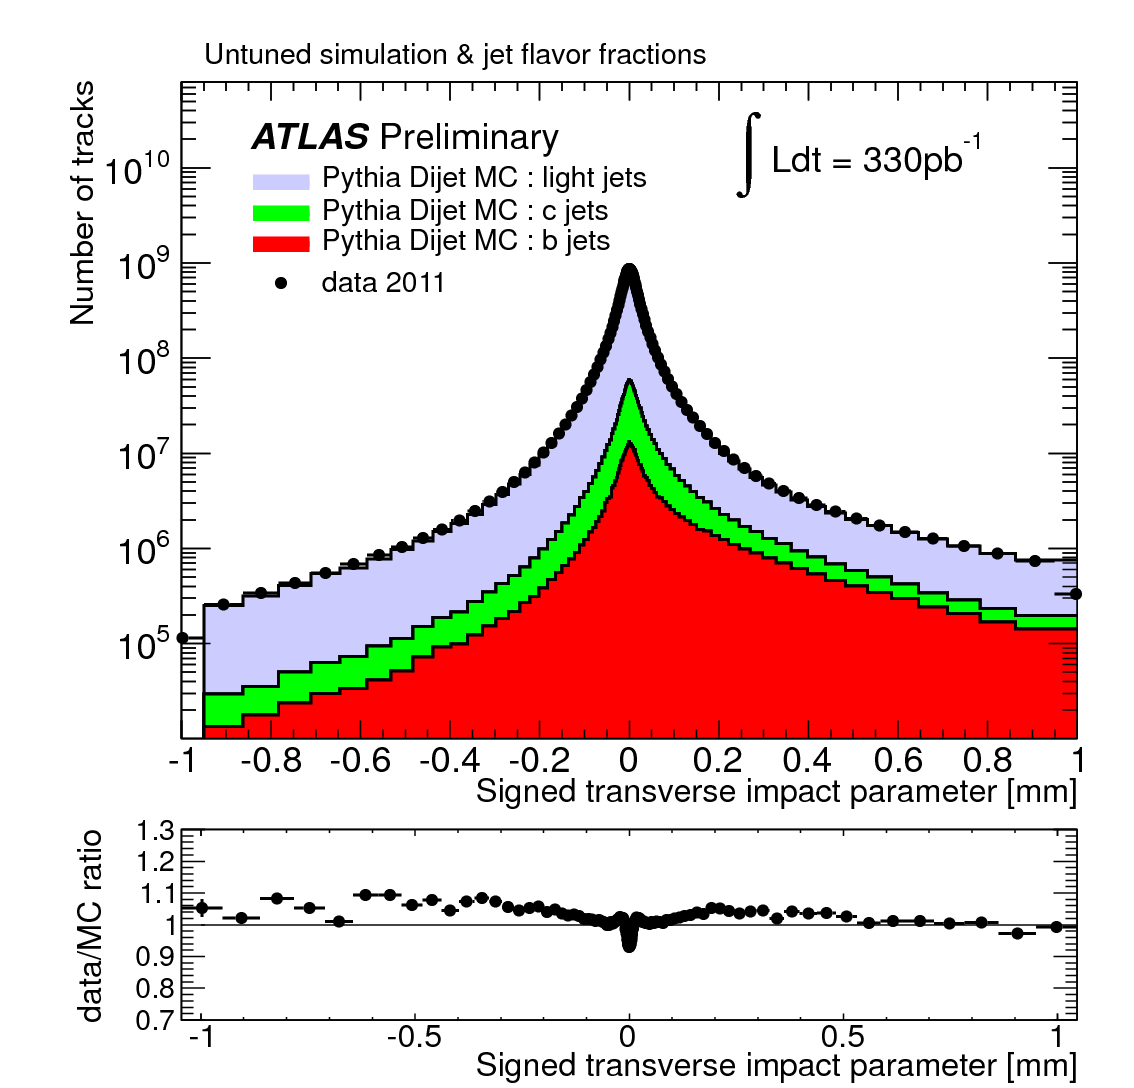
\includegraphics[width=0.49\textwidth]{IP.png}
    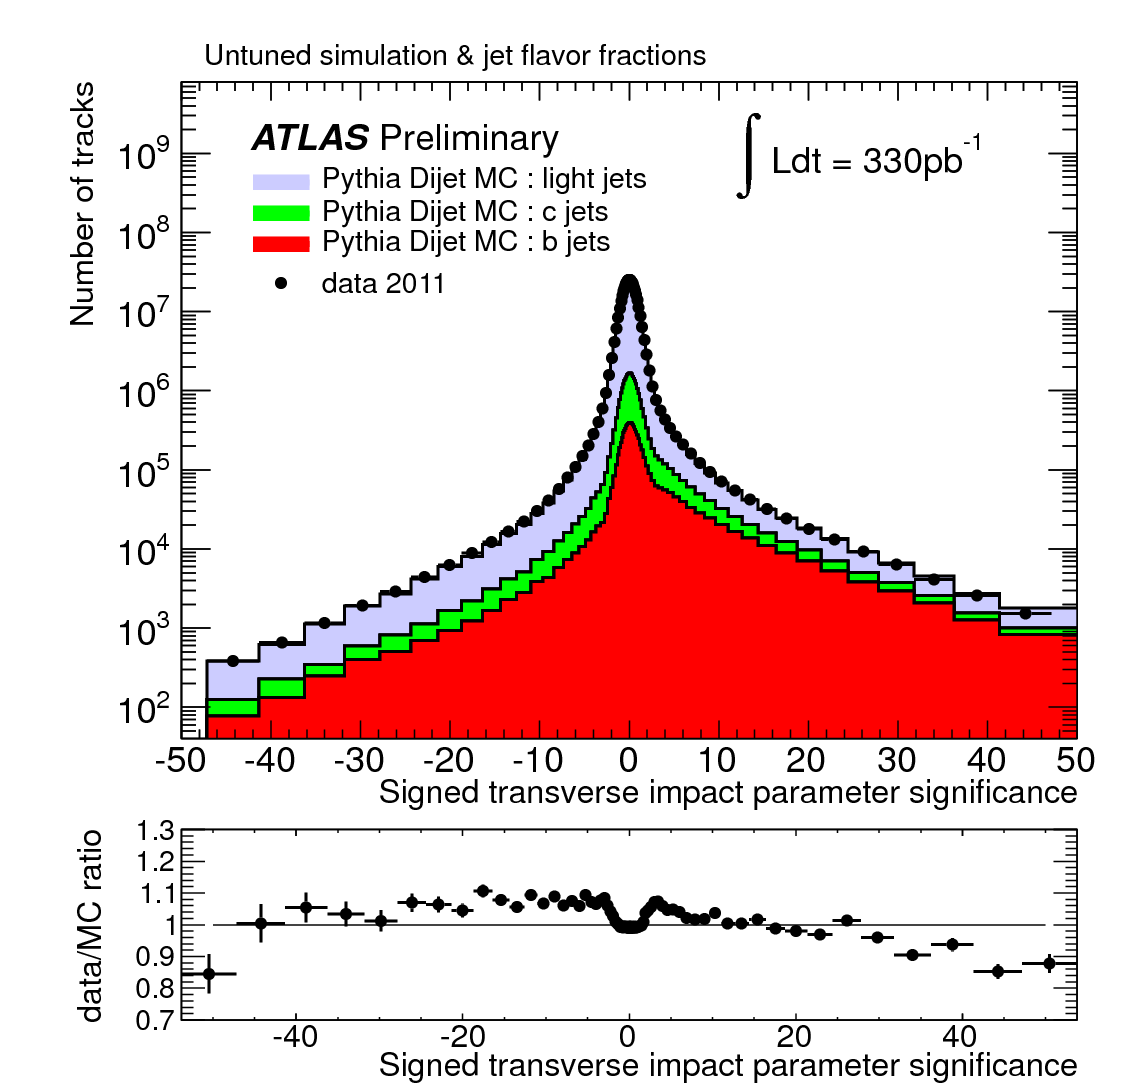
\includegraphics[width=0.49\textwidth]{IPsignificance.png} 
    \caption{Distribution of the signed transverse impact parameter (left) and signed transverse impact parameter significance with respect to primary vertex for tracks associated to jets, for experimental data (solid black points) and for simulated data (filled histograms for the various flavors). The ratio data over simulation is shown at the bottom of the plot.}
    \label{fig:IPsignificance}
  \end{center}
\end{figure}

The significance, which gives more weight to tracks measured precisely, is the main ingredient of the tagging algorithms based on impact parameters. Now, the impact parameter significance of all $N$ tracks associated to the jet to tag need to be combined into a single discriminating variable. It is assumed that tracks are uncorrelated, so their probability density functions (PDF), defined based on the transverse and/or longitudinal impact parameter significance distributions for the different hipothesis, are uniquely  defined as a function of the jet flavour. Using a likelihood function defined according to the product of these PDFs, under the hypothesis of uncorrelated tracks, the following likelihood ratio provides the optimal separation, according to Neyman-Person lemma~\cite{1933RSPTA.231..289N}:
%
\begin{equation}
\mbox{LR}(IP_1,IP_2,...,IP_N) = \frac{\prod_{i=1}^N \mbox{PDF}_b(IP_i)}{\prod_{i=1}^N \mbox{PDF}_l(IP_i)}
\end{equation}
%
For convention, the discriminant variable used for $b$-tagging is then defined as:
%
\begin{equation}
\mbox{weight}(IP_1,IP_2,...,IP_N) = \log(\mbox{LR}(IP_1,IP_2,...,IP_N))
\end{equation}
%
Using such a formalism, two impact parameter based $b$-tagging algorithms are constructed, based on the definition of PDF($IP_i$):

%\begin{itemize}
\begin{enumerate}\addtolength{\itemsep}{-0.4\baselineskip}
\item
IP2D: PDF($IP_i$) = PDF($IP_{i,r\phi}$)
\item
IP3D:  PDF($IP_i$) = PDF($IP_{i,r\phi}$,$IP_{i,z}$)
\end{enumerate}

In the first case the track PDF is one-dimensional, based on the transverse impact parameter significance. In the second case the PDF is based on a two-dimensional histogram of the transverse and longitudinal impact parameter significance. 
%PLOTS OF THE WEIGHTS?

The \textbf{IP3D} is one of the high-performance tagging algorithms supported for the 2011 data-taking, in which input variables are compared to pre-defined smooth Monte Carlo PDFs for both $b$-jet and light jet hypotheses~\cite{ATLAS-CONF-2011-102}.  Prior to the use of these advanced tagger, a simpler tagging algorithm, the \textbf{JetProb}, combining the impact parameter significances of all tracks associated to the jet was devised to be used for early data, being extensively used during 2010~\cite{ATLAS-CONF-2010-091}. 


The impact parameter based algorithm permits to obtain a very good $b$-tagging performance, as will be shown at the end of this chapter. 
%One of the reason of the good performance is that the likelihood method contains implicity, as a prior knowledge in the PDF for $b$-jets, the fraction of tracks expected to arise from fragmentation and the fracion expected to arise from $b$ and $c$-hadron decays. This Method has also a few drawbacks. One is that it does not account for the momentum dependence of the PDFs. And the second is that, while the impact parameter as such is nearly invariant under Lorentz boosts of the $b$-hadron, the error decreases with increasing track $\pt$ and smaller $\eta$. The track-based PDF is thus not invariant neither under a boost of the $b$-quark nor under a boost of its emerging charged particle tracks.This can be cured both by making a track-PDF category dependent. This approach was tried out in ATLAS with significant improvement in performance, but has the disadvantage of increasing the number of free parameters of the likelihood model and making an eventual calibration on data more difficult.
This performance can be improved by using some information from the secondary vertex based algorithms in two aspects: tracks associated to long lived particle vertices can be removed from the tracks considered for the impact parameter based algorithms; and, the direction between the secondary and the primary vertex positions can be used to improve the reliability of the lifetime sign, subtituting $\vec{p}_{jet}$ with $\vec{r}_{SV} - \vec{r}_{PV} $. The latter improves significantly the estimation of the $b$-hadron direction. Both kinds of information improve the performance of the impact parameter based $b$-tagging algorithms.


\subsubsection{Secondary vertex based $b$-tagging algorithms }

The typical topology of particle decays in a $b$-jet is a decay chain with two vertices, one stemming from the $b$-hadron decay and at least one from $c$-hadron decays. The reconstruction of these secondary vertices is done in an inclusive way, where the number of charged particle tracks originating from the $b$- and $c$-hadron decays is not known a-priori. An exclusive reconstruction of the huge number of different possible $b$-decay modes cannot be performed, the set of selection cuts needed to reconstruct all of them would severely limit the reconstruction efficiency.

Two strategies to detect a secondary decay vertex in $b$-jets are available in ATLAS. The first one is based on the fit of a single geometrical vertex. Even if this hypothesis is not correct, this approximation works well for a large fraction of cases.  The second algorithm is based on a kinematic approach, which assumes that the primary event vertex and the $b$- and the $c$-hadron decay vertices lie approximately on the same line, the flight path of the $b$-hadron. 

The inclusive fit of a single displaced vertex in $b$-jets is based on the VKalVrt~\cite{Kostyukhin:685551} reconstruction package. The main idea of the algorithm %implemented in this  package 
is to maximise the $b/c$-hadron vertex detection efficiency, keeping at the same time the probability to find a vertex inside a light jet low. 

The algorithm begins with all tracks associated to the jet and passing a loose cut selection. The vertex search starts with looking for all track pairs and trying to form a two-track vertex. Each track of the pair must have a three-dimensional impact parameter significance with respect to the primary vertex larger than 2$\sigma$ and the sum of these two significances must be larger than 6$\sigma$. To reduce the influence of badly measured tracks, the two-tracks vertices are required to be produced in the direction of flight of the $b$-quark, by requiring the scalar product of $(\vec{r}_{2-track} - \vec{r}_{PV})\cdot \vec{p}_{jet} $ to be positive. Charged particles coming from long lived particles and conversions are not considered.  %for the inclusive $b$-decay vertex fit. 
All the tracks corresponding to the accepted two-track vertices are used to determine a single secondary vertex.  If the resulting vertex has a very small vertex probability, the track with the highest contribution to the vertex $\chi^2$  is removed and the vertex fit is repeated until the $\chi^2$ of the fit is good. The result of this procedure is the (eventual) presence of a vertex, its position, and the list of associated tracks.

The \textbf{SV1} secondary vertex algorithm uses this procedure to reconstruct inclusive secondary vertices. This advanced tagger takes advantage of three of the reconstructed vertex properties: the invariant mass of all tracks associated to the vertex, the ratio of the sum of the energies of the tracks in the vertex to the sum of the energies of all tracks in the jet, and the number of two-track vertices. These variables are combined using a likelihood ratio technique. SV1 relies on a two-dimensional distribution of the two first variables and a one-dimensional distribution of the number of two-track vertices. In addition the distance $\Delta R$ between the jet axis and the line joining the primary vertex to the secondary one is used. 

The three-dimensional decay length significance alone,  signed with respect to the jet direction can be used as a discriminating variable between $b$-jets and light jets: this is the principle of the early data \textbf{SV0} tagger, extensively used as well with the 2010 and 2011 data~\cite{ATLAS-CONF-2010-042}.


As opposed to the algorithm described above, in which the displaced tracks are selected and an inclusive single vertex is obtained, a second algorithm, called \textbf{JetFitter}, is based on a different hypothesis. It assumes that the $b$- and the $c$-hadron decay vertices lie on the same line defined through the $b$-hadron flight path. All charged particle tracks stemming from either decay intersect this $b$-hadron flight axis. This method has the advantage of reconstructing incomplete topologies, with, for instance, a single track from the $b$-hadron and a single track from the $c$-hadron decay. The fit in this case evaluates the compatibility of the given set of tracks with a $b$-$c$-hadron like cascade topology, increasing the discrimination power against light quark jets.
The transversal displacement of the $c$-hadron decay vertex with respect to the $b$-hadron flight path is small enough not to violate significantly the basic assumption within the typical resolutions of the tracking detector.
The discrimination between $b$-, $c$- and light jets is based on a likelihood using similar variables as in the SV1 tagging algorithm above, and additional
variables such as the flight length significances of the vertices.

\subsubsection{Algorithm combinations and performance}

The IP3D and SV1 tagging algorithms both use the likelihood ratio method, and due to this they can be easily combined: the weights of the individual tagging algorithms are simply summed up. 

The combination of the JetFitter and the IP3D algorithms can be performed using an artificial neural network technique with Monte Carlo simulated training samples and additional variables describing the topology of the decay chain. 

Figure~\ref{fig:btaggingperformance} compares the performance for the various ATLAS $b$-tagging algorithms described in a simulated sample of $t\bar{t}$ events.
It can be seen that by combining the vertexing techniques and the impact parameter information, the IP3D+SV1 and IP3D+JetFitter algorithms can reach very high tagging efficiencies.

 The performance of a $b$-tagging algorithm is usally  measured in terms of the \emph{light-jet rejection} obtained for a given \emph{$b$-jet tagging efficiency}.  Curves are obtained by varying continuously the \emph{operating point} of each tagger, i.e. the cut on its output discriminating variable (weight).  The $b$-jet tagging efficiency,  $\epsilon_b$,  is the fraction of jets labeled as $b$-jets that are properly tagged while the light-jet rejection, defined as $1/\epsilon_{light}$, is the reciprocal of the fraction of jets that are labeled as light jets and are actually incorrectly tagged by the algorithm. 

The labeling procedure used for $b$-tagging is based on the flavor of true quarks: a jet is labeled as a $b$-quark jet if a $b$-quark is found in a cone of size $\Delta R = 0.3$ around the jet direction.  The various labeling hypotheses are tried in this order: $b$ quark, $c$ quark and $\tau$ lepton. When none of these hypotheses are satisfied, the jet
is labeled as a light jet. No attempt is made to distinguish light jets originating from gluons from those originating from quarks at this stage.

\begin{figure}[htbp]
  \begin{center}
      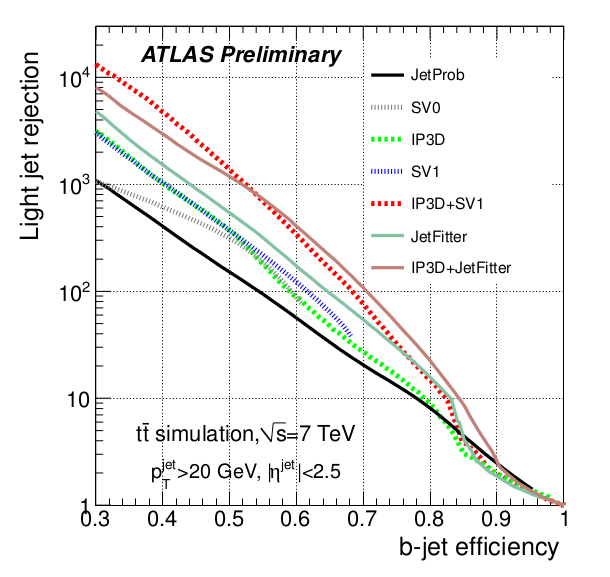
\includegraphics[width=0.7\textwidth]{btaggingperformance.png}
    \caption{Light-jet rejection as a function of the $b$-jet tagging efficiency for the early tagging algorithms (JetProb and SV0) and for the high-performance algorithms, based on simulated $t\bar{t}$ events. }
    \label{fig:btaggingperformance}
  \end{center}
\end{figure}

%By combining the vertexing techniques and the impact parameter information, the IP3D+SV1 and IP3D+JetFitter algorithms can reach very high tagging efficiencies.


\subsubsection{The MV1 tagging algorithm}


The \textbf{MV1} $b$-tagging algorithm is a combined algorithm based on a neural network using the output weights of the IP3D and SV1 algorithms and the JetFitter+IP3D combination as input.  Being the best performing algorithm (better light rejection for a given signal efficiency) it is the recomended tagger for 2011 and 2012 analyses. This is the $b$-tagging algorithm used in this thesis.

%%PLOT OF THE MV1 WEIGHT???????????????
%%TABLA DE LOS SUPPORTED OPERATING POINTS????????

\subsection{$b$-tagging calibration}


In order for $b$-tagging to be used in physics analyses, the efficiency with which a jet originating from a $b$-quark is tagged needs to be measured in data.  Moreover, an appropriate description of the $b$-tagging efficiencies based on measurements with data is essential for correctly modelling the measurements in Monte Carlo simulation . A second necessary piece of information is the probability of mistakenly tagging a jet originating from a light-flavour ($u$-, $d$-, $s$-quark or gluon) jet as a $b$-jet, referred to as the mistag rate. The $b$-tagging ``calibration'' includes both the measurement of the mistag rates and $b$-tagging efficiency.


The measurements of the $b$-tag efficiency and mistag rate are provided in the form of jet $\pt$- and $\eta$-dependent scale factors that correct the $b$-tagging performance in simulation to that observed in data.  The scale factors are defined as the ratio of the $b$-tag efficiency or mistag rate in data and simulation:
%
\begin{equation}
\kappa_{\epsilon_b}^{data/sim}  = \frac{\epsilon_b^{data}}{\epsilon_b^{sim}}, \; \;   \kappa_{\epsilon_l}^{data/sim}  = \frac{\epsilon_l^{data}}{\epsilon_l^{sim}},
\end{equation}
%
where $\epsilon_b^{sim}$ and $\epsilon_l^{sim}$ are the fractions of $b$- and light-flavour jets which are tagged in simulated events, %an inclusive sample of simulated $t\bar{t}$ events,
 with the jet flavour defined by matching to generator level partons as defined in the previous section. %The measured $b$-tag efficiencies and mistag rates will depend on the jet transverse momentum $\pt$ and the pseudorapidity $\eta$.  %They also depend on other quantities such as the fraction of jets in the sample originating from gluons. An advantage of providing the calibration results in the form of scale factors is that even though samples with different event topologies can have slightly different $b$-tag efficiencies or mistag rates, the data-to-simulation scale factors are likely to be valid.

In physics analyses, these $\pt$-dependent scale factors are then applied as weights to the jets in Monte Carlo simulation, to reproduce the $b$-tagging performance in data.


The main $b$-tagging efficiency calibration methods, the so called \emph{system8} and $\pt_{rel}$ methods, are described in detail in ref~\cite{ATLAS-CONF-2011-089}.% based on an integrated luminosity of L = 4.7 fb−1 collected in 2011. 
These measurements are based on a sample of jets with muons inside, where the muons are serving as a reference $b$-tagging algorithm to obtain a $b$-jet sample on which the calibrations can be performed. 
At the LHC, the large $t\bar{t}$ production cross section of $\sigma_{t\bar{t}} = 177 \pm 3(\mbox{stat.})  \; _{-7}^{+8} (\mbox{syst.}) \pm 7(\mbox{lum.})$~pb~\cite{ATLAS-CONF-2012-024} offers an alternative source of events enriched in $b$-jets. % This distinctive topology with high pT leptons, multiple jets, and large missing transverse momentum provides highly selective trigger objects and is relatively easy to reconstruct. With the large integrated luminosity of 4.7 fb−1 collected during 2011, the methods based on tt selections have become competitive for the first time. In addition to providing b-tagging calibration measurements in an inclusive b-jet sample rather than a sample of semileptonic b-jets. In addition to providing b-tagging calibration measurements in an inclusive b-jet sample rather than a sample of semileptonic b-jets, these methods  methods also allow to extend the calibrated pT range. Furthermore, the tt environment of high jet  multiplicity and high pT b-jets is more similar to the final states to which b-tagging is applied than the semileptonic jet sample.
Calibrations using samples of $t\bar{t}$ events have been obtained for SV0, IP3D+SV1, JetFitter and MV1 $b$-tagging algorithms~\cite{ATLAS-CONF-2012-097}. All these algorithms provide an output weight $w$, discriminating between $b$-jets and non-$b$-jets. Lower values of $w$ are assigned to $c$- and light-flavour jets, whereas the purity of $b$-jets increases with $w$. For each $b$-tagging algorithm a set of operating points, corresponding to a certain $w$ cut value, are defined and calibrated:

\begin{itemize}
\item
SV0: $\epsilon_b^{sim} =$ 50\%
\item
IP3D+SV1: $\epsilon_b^{sim} =$ 60\%, $\epsilon_b^{sim} =$ 70\%, $\epsilon_b^{sim} =$ 80\%
\item
JetFitter: $\epsilon_b^{sim} =$ 57\%, $\epsilon_b^{sim} =$ 60\%,  $\epsilon_b^{sim} =$ 70\%, $\epsilon_b^{sim} =$ 80\%
\item
MV1: $\epsilon_b^{sim} =$ 60\%, $\epsilon_b^{sim} =$ 70\%, $\epsilon_b^{sim} =$ 75\%, $\epsilon_b^{sim} =$ 85\%
\end{itemize}
%
where  $\epsilon_b^{sim}$ is the nominal $b$-tagging efficiency derived from an inclusive sample of simulated $t\bar{t}$ events.

%http://cdsweb.cern.ch/record/1435194
The mistag rate is measured in data using two methods, both based on an inclusive sample of jets, referred to as the $negative tag$ and $sv0mass$ methods~\cite{ATLAS-CONF-2012-040}. The first method uses the invariant mass spectrum of tracks associated with reconstructed secondary vertices to separate light and heavy-flavour jets, and the other is based on the rate at which secondary vertices with negative decay length, or tracks with negative impact parameter, are present in the data.


Currently, there is no explicit measurement of the $c$-tag efficiency available in ATLAS. As both the
$b$- and $c$-tag efficiencies are dominated by decays of long-lived heavy flavour hadrons, they are expected to show a similar behaviour. In general, for physics analyses, it is thus assumed that the scale factor is the same for $b$- and $c$-jets. However, to take into account possible deviations from this assumption, the systematic uncertainty for the $c$-tag efficiency scale factor is inflated by a factor of two, which is considered to be a conservative choice based on simulation studies. In the future, the $c$-tag efficiency is expected to be measured in dedicated analyses.



%\subsection{Pile-up}
%Out-of-time pile-up events ($pp$ collisions from neighboring bunches in the same train) also generate calorimeter activity and consequently extra jets. However, given the time resolution of the Inner Detector, and since the $b$-tagging algorithms reject jets with no track associtaed to them, the contribution of the out-of-time pile-up for this analysis is expected to be negligible.
